\chapter{Edges}
\begin{figure}
    \centering
    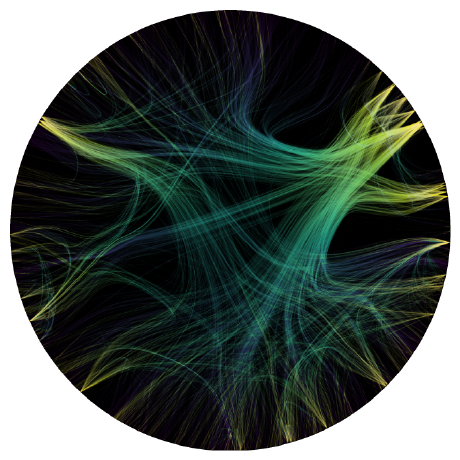
\includegraphics[width=.6\textwidth]{power/figures/metaunityplaceholder.png}
    \caption{A visualisation of the Unity game engine, produced using the Unity game engine.}
    \label{fig:metaunity}
\end{figure}
The previous chapter of was an exploration of how to position the nodes of a graph, and the natural question to then ask is how to deal with the only remaining component: the links. However this question is seemingly redundant at first, as the obvious answer is to simply draw straight lines between nodes with edges between them. While this by no means a poor choice, and is exactly how all node-link diagrams have been drawn thus far, this chapter will explore the possibility of drawing links using curves instead.

\section{Background}
The curving of links in the context of a node-link diagram is known as \textit{edge bundling}. It is a technique that has been developed because many networks, when processed through a standard force-directed layout, result in a seemingly random layout with no discernable structure. See Figure~\ref{TODO} for an example. The similarity of such layouts to tangled piles of hair has led to them being colloquially termed \textit{hairballs}.

Unfortunately this is not an easily solved problem, because the \textit{curse of dimensionality}~\cite{TODO} means that most of these networks simply cannot be accurately represented in two dimensions, and the likelihood of this problem only rises as the size of any network increases. This is all even if there is a clear underlying structure to these networks, lying beyond the reach of the standard layout algorithm.
Edge bundling attempts to alleviate this issue by introducing a trade-off---the ability to follow individual links is sacrificed for better representation of global structure, by allowing links to overlap.

This is analogous to organising the wires in a computer system by tying groups of wires together that share similar endpoints. A simple example of this is illustrated in Figure~\ref{TODO}, where the compromise between being able to follow links showing global structure is clearly visible.

The literature is rich with various different methods for performing this bundling, such as multilevel agglomerative edge bundling (MINGLE) by Gansner et al.~\cite{TODO} which greedily merges pairs of links at a time by selecting the pairs that minimise a cost function based on the amount of `ink' used to draw links. A more complex cost function is used in metro-style bundling by Pupyrev et al.~\cite{TODO}, which is based on multiple criteria including ink, individual edge lengths and separations. 
The same premise behind force-directed node layout is also used in force-directed edge bundling by Holten~\cite{TODO}, which bundles links by defining forces between adjacent links instead of nodes. However, as shown previously in Section~\ref{TODO}, force-based methods are in fact gradient descent optimisation methods where the gradient is defined before the cost function itself, and this edge bundling technique is no different.

A slightly different but effective approach comes from Kernel Density Estimation by Hurter et al.~\cite{TODO}, who iteratively apply a convolutional filter over a density map of links in an already rendered diagram, and has spawned the subfield of image-based bundling methods~\cite{TODO,TODO,TODO}.
However all of the aforementioned methods share a key similarity: they apply bundling upon the assumption that node positions are predetermined and will not be moved. This is perfectly fine and in fact desirable in the case of many common use cases, such as geographical maps etc. but by definition do not take the actual structure of the data into account. Force-directed layouts, in particular, were never designed to place similar edges in parallel (in fact, edge angular resolution at nodes is even sometimes used as part of the cost function~\cite{TODO}) and so common force-directed layouts do not necessarily help, if not make worse, the bundling quality of a visualisation.

This is why one of the most powerful graph visualisations is technique known as hierarchical edge bundling, published by Holten in 2006~\cite{TODO}. The reason behind its effectiveness is that it uses extra metadata in order to inform the nature of the bundling; specifically every vertex in the visualised graph also exists as a leaf vertex in a hierarchical tree. As an example, a common and effective use case is in the call graph of a piece of software. Each function is a vertex, and is connected by an edge to any other function that calls it. The metadata in this case is the hierarchy of folders and source files within.
An example of this technique can be seen in Figure~\ref{fig:metaunity}, which contains this visualisation applied to the source code of the Unity game engine. The hierarchical tree itself can be seen on the TODO hand side, to illustrate the layout and influence of the ARG on the final visualisation. 

The trick to the bundling is as follows: the hierarchy, not the call graph itself, is first layed out as a tree. Then, since this tree contains extra nodes to represent the folders and source files, these extra nodes are erased from the final visualisation. They are instead used as an auxiliary routing graph (ARG) through which the call graph edges are routed through.
More precisely, this process of routing involves taking every edge in the call graph, and rendering each one using a spline curve whose control points consist of a path through the ARG. The precise definition of this spline is important, and will be further elaborated upon in Section~\ref{TODO}, but for now the important thing to note is that this produces bundling behaviour because vertices close to each other in the hierarchy will often share control points for their splines, to curve their rendered links towards each other.

This technique is so effective because the structure of the bundles is informed by human judgement. To continue within the call graph example, the hierarchy of folders and source files is literally designed by the programmers for organisational purposes, and so it is very likely to admit some utility for organising, say, a visualisation.
This idea of using an auxiliary graph to inform bundling is the basis of the work in this chapter, except that I will instead investigate the more common situation of when this metadata is not included with the original data, and therefore must be inferred instead.

\section{Hierarchical Clustering}
What is needed is a method for of grouping similar datapoints together. This is known as \textit{clustering}, and is a vast field of study, not least as one of the primary objectives of the fast-growing discipline of machine learning. The subfield of clustering within the context of networks is large in its own right, due to its utility in common datasets such as protein--protein interaction or social networks.

There exist a wide variety of powerful and creative methods that have been developed to perform clustering on networks. A common 
Louvain (given its name from the authors coming from the University of Louvain, Belgium) and its recently updated Leiden (Leiden University, Netherlands) attempt to optimise a cost function known as \textit{modularity}, which was developed by...
Modularity has problems such as resolution limit... CPM can avoid this
Random walks are a popular the Infomap algorithm optimises a cost function known as the map equation, which (like pagerank) with a combination of greedy search and simulated annealing.
and markov cluster...
link clustering

% The variety of different methods available is in part due to one key characteristic of network clustering: it is an undefined problem.
One reason why there is such a variety of clustering algorithms is in part due to it being an inherently difficult problem.
Clustering can be likened to data compression, as the goal is to describe a given network with less information than, say, viewing the source and target of every individual edge. Such compression would be impossible in a random network, but because real-world data does have structure, underlying patterns can be leveraged to group together similar components within the data.
However, even knowing that this is the goal does not make the problem easier, because these underlying patterns are not known to us. The real world is complex, and so any data collected from it is not likely to be straightforward to understand. Much of the data collected may not even contain any order in the first place.
% In fact, if you will allow me to go meta for a moment, the very act of collecting data itself into the form of a network is already technically a form of compression, as 
It is therefore important to keep in mind that all metrics like the aforementioned modularity or map equation are simply attempts to quantify common characteristics of real-world data, and there is no `right answer' to the question of which one should be chosen. It depends on both the specific objective and dataset being examined. Nevertheless, they have been used to great effect in many applications~\cite{TODO}, and so confidence can be placed in their utility as a tool to help understand patterns in data.

The work in this chapter will concentrate on \textit{agglomerative clustering}, which is a family of algorithms that starts by placing each datapoint in a separate cluster, and then proceeds by merging clusters together. 
The benefit of this method is that the output is a \textit{dendrogram}, which is a binary tree that describes a hierarchical structure. Each branch in the tree represents a merge between two clusters, and the root therefore represents a single cluster containing the entire dataset. To perform the desired hierarchical edge bundling, as the name suggests, requires a hierarchy with multiple levels, not just a set of clusters, and so the output of an agglomerative clustering algorithm can be used directly as the hierarchical metadata needed.

% Another benefit to agglomerative methods is that it is easy to interpret and understand what the algorithm is doing. I would always pick an algorithm that I fully understand for a visualisation over a black-box algorithm that produces slightly better results. But this is just opinion.
Within agglomerative clustering there are 
NP-hard problem blah blah
Unweighted is, perhaps confusingly, more precise than the weighted version (directly opposite to the case in weighted and unweighted shortest paths). 
UPGMA WPGMA ward is better because of things

% it is very important to realise that there are two types of clusters, which will be henceforth referred to as 'community' and 'betweenness' structure. This can also be referred to as 'assortative' and 'disassortative'.
% some networks have both at the same time, and it is therefore difficult

The idea of generating a hierarchy from the data was previously explored by Jia et al.~\cite{TODO}\footnote{bad splines}, who produce a hierarchy using a method known as \textit{divisive clustering} by Girvan and Newman~\cite{TODO}. This method also forms a dendrogram, but in the reverse order: it starts with one big cluster and iteratively splits it in order to form the dendrogram from the top-down instead of bottom-up. This divisive method specifically removes one edge from the network at a time, which naturally splits clusters when the removal of an edge leads to components being separated from each other. The problem with this method can be seen in figure~\ref{TODO} will be discussed in the following section, where I will present an exploration of the agglomerative methods we require. 

\subsection{Distance measures}

mention the optimal ordering from Scipy, Bar-Joseph et al.~\cite{TODO}, around a circle

try WASSERSTEIN

\begin{itemize}
    \item girvan-newman -- this results in long strands that \item
\end{itemize}

\section{Power-confluent Drawings}
in confluent drawings the aforementioned trade-off is actually attempted to be avoided
it is likened to lossless compression.
fixing issues and improving speed
\subsection{Splines}
b-spline algorithms and things
holten qualitatively said some desirable properties of b-splines, but the real benefit of them is the convex hull property, which helps to prevent crossings (explain why... because)
The importance of this has been crucially missing in the literature
examples of splines that are not convex hull is like the garland paper.
